\documentclass[20pt,landscape,a0paper]{tikzposter}

\usepackage[american]{babel}
\usepackage[utf8]{inputenc}
\usepackage[T1]{fontenc}
\usepackage{amsmath,amssymb}
\usepackage{tikzsymbols}
\usepackage{wrapfig}
\usepackage{tikz}
\usetikzlibrary{matrix,arrows,arrows.meta,bending,positioning}
\tikzset{>/.tip={Computer Modern Rightarrow[scale=2,line width=1pt]}}
\tikzset{|/.tip={Bar[scale=2,line width=1pt]}}

\def\Q {\ensuremath{\mathbb{Q}}}
\def\Z {\ensuremath{\mathbb{Z}}}
\def\F {\ensuremath{\mathbb{F}}}
\def\Tr {\ensuremath{\mathrm{Tr}}}
\def\M {\ensuremath{\mathsf{M}}}
\def\tildO {\ensuremath{\mathrm{\tilde{O}}}}

\renewcommand{\paragraph}[1]{\smallskip\textbf{#1}}
\colorlet{alert}{red}

\title{Computing isomorphisms and embeddings of finite fields}
\author{Ludovic Brieulle\footnotemark[1], Luca De Feo\footnotemark[1],
  Javad Doliskani\footnotemark[2], Jean-Pierre Flori\footnotemark[3],
  Éric Schost\footnotemark[2]} \institute{\footnotemark[1]Université
  de Versailles -- Saint-Quentin-en-Yvelines,
  \footnotemark[2]University of Western Ontario,
  \footnotemark[3]Agence Nationale de Sécurité des Systèmes
  d'Information}

\usetheme{Desert}

\begin{document}
\maketitle

\begin{columns}
  %%%%%%%%%%%%%%%%%
  % Intro
  %%%%%%%%%%%%%%%%%
  \column{0.25} \block{The embedding problem}{
    \begin{wrapfigure}{r}{0.45\colwidth}
      \centering
      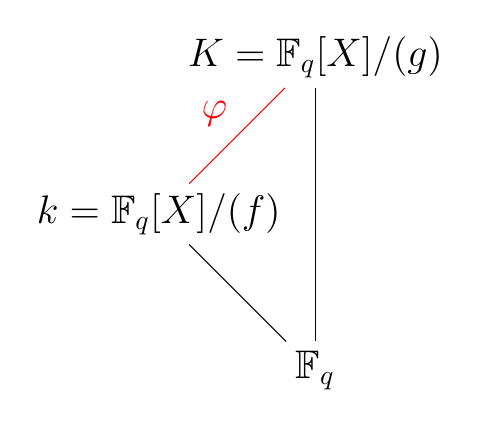
\begin{tikzpicture}[node distance=8em,font=\Large]
        \node(Fq){$\F_q$};
        \node(Fqf)[above left of=Fq]{$k=\F_q[X]/(f)$};
        \node(Fqg)[above right of=Fqf]{$K=\F_q[X]/(g)$};
        \draw[]
        (Fq) edge (Fqf)
        (Fq) edge (Fqg)
        (Fqf) edge[left,auto,color=alert] node{$\varphi$} (Fqg);
      \end{tikzpicture}
    \end{wrapfigure}

    \paragraph{Let}
    \begin{itemize}
    \item $\F_q$ be a field with $q$ elements,
    \item $f$ and $g$ be irreducible polynomials in $\F_q[X]$,
    \item $m=\deg f$, $n=\deg g$ and $m|n$.
    \end{itemize}

    There exists a field
    embedding \[\color{alert}\varphi:k\hookrightarrow K,\] unique up to
    \mbox{$\F_q$-auto}morphisms of $k$.

    \paragraph{Goals}
    \begin{itemize}
    \item \textbf{Represent} $\varphi$ efficiently,
    \item \textbf{Evaluate/Invert} $\varphi$ efficiently,
    \end{itemize}

    When $\deg f = \deg g$, this is also called the
    \emph{isomorphism problem}. 
    
    \paragraph{Applications}
    \begin{itemize}
    \item Fundamental building blocks of computer algebra systems.
    \item Work algorithmically in the algebraic closure
      $\bar{\F}_q$~\cite{bosma+cannon+steel97}.
    \end{itemize}
  }

  \block{Embedding description}{ 
    \begin{wrapfigure}[8]{r}{0.4\colwidth}
      \centering
      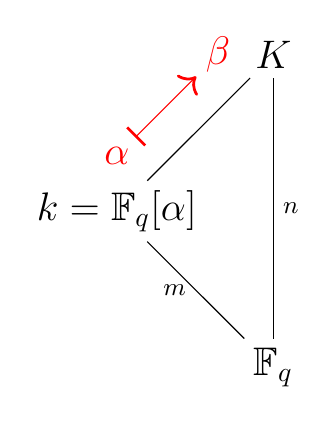
\begin{tikzpicture}[node distance=8em,font=\Large]
        \node(Fq){$\F_q$};
        \node(Fqf)[above left of=Fq]{$k=\F_q[\alpha]$};
        \node(Fqg)[above right of=Fqf]{$K$};
        \begin{scope}[alert,node distance=2em]
          \node(a)[above of=Fqf]{$\alpha$};
          \node(b)[left of=Fqg]{$\beta$};
        \end{scope}
        \draw[auto,font=\small]
        (Fq) edge node[left]{$m$} (Fqf)
        (Fq) edge node[right]{$n$} (Fqg)
        (Fqf) edge (Fqg);
        \draw[|->,alert]
        (a) edge (b);
      \end{tikzpicture}
    \end{wrapfigure}

    \textbf{Determine} elements $\alpha\in k$ and $\beta\in K$ such
    that

    \begin{itemize}
    \item $\alpha$ generates $k=\F_q[\alpha]$,
    \item there exists $\varphi:\alpha\mapsto\beta$.
    \end{itemize}

    \paragraph{Naive solution:} take
    \begin{itemize}
    \item $\alpha= X \mod f(X)$, and
    \item $\beta$ a root of $f$ in $K$.
    \end{itemize}
    Cost of factorization: $\tildO(mn)$.\\ Storage: $O(n)$.

    \paragraph{Kummer-type algorithms}: Use properties of $m$-th
      roots of unity.
    \paragraph{Group-based algorithms}: Use properties of an
      algebraic group $G/\F_q$.
  }

  \block{Embedding evaluation}{ 
    \begin{wrapfigure}[8]{r}{0.2\colwidth}
      \centering
      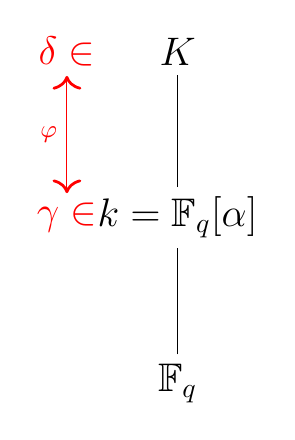
\begin{tikzpicture}[node distance=6em,font=\Large,on grid]
        \node(Fq){$\F_q$};
        \node(Fqf)[above=of Fq]{$k=\F_q[\alpha]$};
        \node(Fqg)[above=of Fqf]{$K$};
        \begin{scope}[alert,node distance=4em]
          \node(a)[left=of Fqf]{$\gamma\in$};
          \node(b)[left=of Fqg]{$\delta\in$};
        \end{scope}
        \draw
        (Fq) edge (Fqf)
        (Fqf) edge (Fqg);
        \draw[<->,alert]
        (a) edge node[left,auto,font=\small]{$\varphi$} (b);
      \end{tikzpicture}
    \end{wrapfigure}

    \textbf{Given}
    \begin{itemize}
    \item a \emph{description} of the embedding (as above),
    \item $\gamma\in k$ and $\delta\in K$,
    \end{itemize}

    \textbf{Solve} the following problems:
    \begin{itemize}
    \item Compute $\varphi(\gamma)$ in $K$.
    \item Test if $\delta\in\varphi(k)$.
    \item Supposing $\delta\in\varphi(k)$, compute $\varphi^{-1}(\delta)$ in $K$.
    \end{itemize}
    
    \textbf{Naive solution:} Linear algebra (size $n\times m$).
  }

  %%%%%%%%%%%%%%%%%
  % Kummer-type
  %%%%%%%%%%%%%%%%%
  \column{0.25}
  
  \block{Lenstra's algorithm~\cite{LenstraJr91}}{
    \begin{wrapfigure}{l}{\colwidth}
      \paragraph{Goals}
      \begin{itemize}
      \item Prove that the isomorphism problem is \emph{deterministic
          polynomial}.
      \item Pervasive use of linear algebra.
      \item Does not prove precise complexity. Rough estimate:
        $\Omega(n^3)$.
      \end{itemize}
    \end{wrapfigure}

    \begin{wrapfigure}[4]{r}{0.45\colwidth}
      \centering
      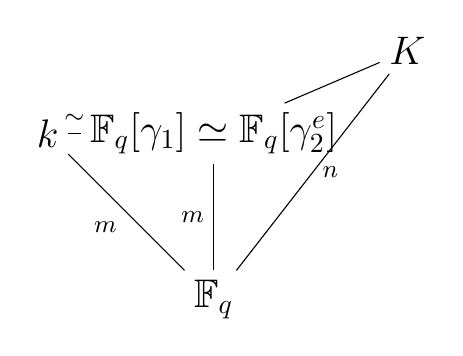
\begin{tikzpicture}[node distance=6em,font=\Large,on grid]
        \node(Fq){$\F_q$};
        \node(kum)[above=of Fq]{$\F_q[\gamma_1]\simeq\F_q[\gamma_2^e]$};
        \node(k)[left=6em of kum]{$k$};
        \node(K)[above right=3em and 7em of kum]{$K$};
        \draw[auto,font=\small]
        (Fq) edge node{$m$} (kum)
        (Fq) edge node{$m$} (k)
        (Fq) edge node[right]{$n$} (K)
        (k) edge node[]{$\sim$} (kum)
        (kum) edge node{} (K);
      \end{tikzpicture}
    \end{wrapfigure}

    \paragraph{Technique}
    \begin{itemize}
    \item Reduce to $n$ a prime power.
    \item If $(n,q)>1$,
      \begin{itemize}
      \item  use Artin-Schreier theory.
      \end{itemize}
    \item Else,
      \begin{itemize}
      \item find $\gamma_1\in k$ s.t. $\gamma_1^m=c_1\in\F_q$,
      \item find $\gamma_2\in K$ s.t. $\gamma_2^m=c_2\in\F_q$,
      \item compute $c_2=c_2^e$, then $\gamma_1\mapsto\gamma_2^e$.
      \end{itemize}
    \end{itemize}

    In general, if $m\nmid(q-1)$, adjoin roots of unity by working in
    \emph{cyclotomic extension rings}.
  
  }

  \block{Allombert's variant~\cite{Allombert02}}{
    \paragraph{Goals}
    \begin{itemize}
    \item Trade determinism for efficiency.
    \item Implementation integrated into Pari/GP.
    \item \textcolor{alert}{Still missing a rigorous complexity
        analysis. \Large\Sadey}
    \end{itemize}
    
    \paragraph{Technical differences}
    \begin{itemize}
    \item Allow factorization of cyclotomic polynomials to construct
      $\F_q[\mu_m]$.
    \item Explicit use of Hilbert '90 to compute $\gamma_1$ and
      $\gamma_2$.
    \item $\gamma_1/\gamma_2$ is in $\F_q[\mu_m]$: compute it by
      taking the $m$-th root of $c_1/c_2$.
    \item \textcolor{alert}{Use linear algebra to solve Hilbert
        '90???}
    \item Use Shank's algorithm to compute $m$-th roots in
      $\F_q[\mu_m]$.
    \item \textbf{Complexity:} $O\left(m^{\omega+1}\right)$ (dominated
      by Hilbert '90).
    \end{itemize}

    \paragraph{Our improvements}
    \begin{itemize}
    \item Classic trick (also present in Lenstra) + \emph{iterated
        frobenius}~\cite{vzgathen+shoup92:journal} to solve Hilbert
      '90 \textbf{efficiently}.
    \item Use factorization~\cite{kaltofen+shoup97} to compute $m$-th
      roots in $\F_q[\mu_m]$.
    \item \textcolor{alert}{Complexity analysis. \Large\Smiley}
    \item \textbf{Complexity:} $\tildO(m^2)$, but very efficient when
      $m\mid(q-1)$.
    \end{itemize}
  }

  %%%%%%%%%%%%%%%%%
  % Group-based
  %%%%%%%%%%%%%%%%%
  \column{0.25}
  \block{Pinch's algorithm~\cite{Pinch}}{
    
  }
  \block{Rain's cyclotomic algoritm~\cite{rains2008}}{
  }
  \block{Elliptic curve variant}{
  }

  %%%%%%%%%%%%%%%%%
  % Embedding evaluation
  %%%%%%%%%%%%%%%%%
  \column{0.25}
  \block{Linear algebra and modular composition}{
    Kedlaya-Umans
  }
  \block{Normal bases}{
    http://www.shoup.net/papers/subquadratic.pdf
  }
  \block{Benchmarks}{}
  \block{\refname}{
    \small
    \renewcommand*{\refname}{\vspace{-1em}}
    \bibliographystyle{plain}
    \bibliography{../defeo}
  }

\end{columns}

\end{document}